\section{Założenia i narzędzia}
\label{ch:zalozenia}
Założenia podzielone zostały na kilka podsekcji, po jednej dla każdej części projektu. Wyjaśnienie poszczególnych części/modułów znajduje się w Rozdziale \ref{ch:project}.

\subsection*{Założenia dla układu elektronicznego}
\begin{itemize}
    \item 2 silniki DC (ang.~\english{Direct Current})
    \item sterownik silników
    \item czujnik laserowy z przodu pojazdu
    \item enkodery optyczne do pomiaru położenia wałów silników
    \item sterowanie przy użyciu mikroprocesora
    \item LED (ang.~\english{Light Emitting Diode}) sygnalizujący stan oprogramowania mikroprocesora
    \item głośnik sygnalizujący stan oprogramowania mikroprocesora
    \item bezpieczniki zabezpieczające układ elektroniczny
    \item przełączniki źródeł prądowych
\end{itemize}

\subsection*{Założenia dla modelu pojazdu}
\begin{itemize}
    \item 4 koła
    \item możliwa jazda do przodu, tyłu oraz skręcanie jak w samochodzie osobowym
    \item kilka rozmiarów kół dla różnorodności eksperymentalnej
    \item modułowość pozwalająca na modyfikację w razie potrzeby
    \item projekt wizualny podobny do samochodu osobowego
    \item w miarę możliwości niska masa
    \item obudowa wydrukowana na drukarce 3D
\end{itemize}

\subsection*{Założenia dla oprogramowania mikroprocesora}
\begin{itemize}
    \item system FreeRTOS (ang.~\english{Real Time Operating System})
    \item wykonanie w języku C++
    \item klient UDP (ang.~\english{User Datagram Protocol})
    \item serwer UDP
    \item interpretacja danych z ramek pakietów UDP
    \item sterowanie możliwe w układzie otwartym lub zamkniętym
    \item wartość zadana odbierana z aplikacji mobilnej przez wifi
    \item rozpoczęcie i zakończenie pomiaru na komendę z aplikacji mobilnej
    \item awaryjne zakończenie pomiaru w przypadku rozłączenia wifi
    \item odczytywanie kierunku i położenia enkoderów
    \item synchronizacja silników
    \item obliczanie sygnałów sterujących silników
    \item regulatory PID
    \item plik konfiguracyjny
\end{itemize}

\subsection*{Założenia dla aplikacji mobilnej}
\begin{itemize}
    \item działanie na systemie Android
    \item prostota wykonania
    \item prostota użytkowania
    \item krótki czas tworzenia (ang.~\english{development})
    \item klient UDP
    \item serwer UDP
    \item interpretacja danych z ramek pakietów UDP
    \item zmienny docelowy adres IP (ang.~\english{Internet Protocol}) 
    \item parametryzacja regulatorów PID
    \item ustawianie wartości zadanej
    \item ustawianie prędkości
\end{itemize}

\subsection*{Założenia dla skryptu odbierającego dane}
\begin{itemize}
    \item działanie na systemie windows
    \item wykonanie w języku Python
    \item serwer UDP
    \item interpretacja danych z ramek pakietów UDP
    \item zapis danych do pliku .csv (ang.~\english{Comma-Separated Values})
    \item działanie w pętli; możliwość odbioru wielu pomiarów
\end{itemize}

\subsection*{Założenia dla skryptu wizualizujacego dane}
\begin{itemize}
    \item działanie na systemie windows
    \item odczytywanie danych z pliku .csv
    \item wizualizacja odczytanych danych (tworzenie wykresów)
    \item zapisywanie wykresów do pliku .eps (ang.~\english{Encapsulated PostScript})
\end{itemize}

\newpage

\section{Narzędzia}
\label{ch:narzedzia}
% ============ hardware ============ %
\subsection*{Narzędzia fizyczne}

\subsubsection*{Zestaw lutowniczy} % kim był Transformatorov?
Lutowanie to proces łączenia elementów elektronicznych przez stopienie spoiwa lutowniczego na przylegających do siebie elementach metalowych, a następnie jego zastygnięcie. Wykorzystane zostały następujące narzędzia:

\begin{itemize}
    \item lutownica transformatorowa 100 W (Rysunek~\ref{fig:lutownica})
    \item topnik w żelu
    \item plecionka do rozlutowywania
    \item cyna lutownicza bezołowiowa z 3.8\% srebra
    \item alkohol izopropylowy 100\%
    \item zestaw przewodów typu prototypowego (ang.~\english{jumper wires})
\end{itemize}

\begin{center}
    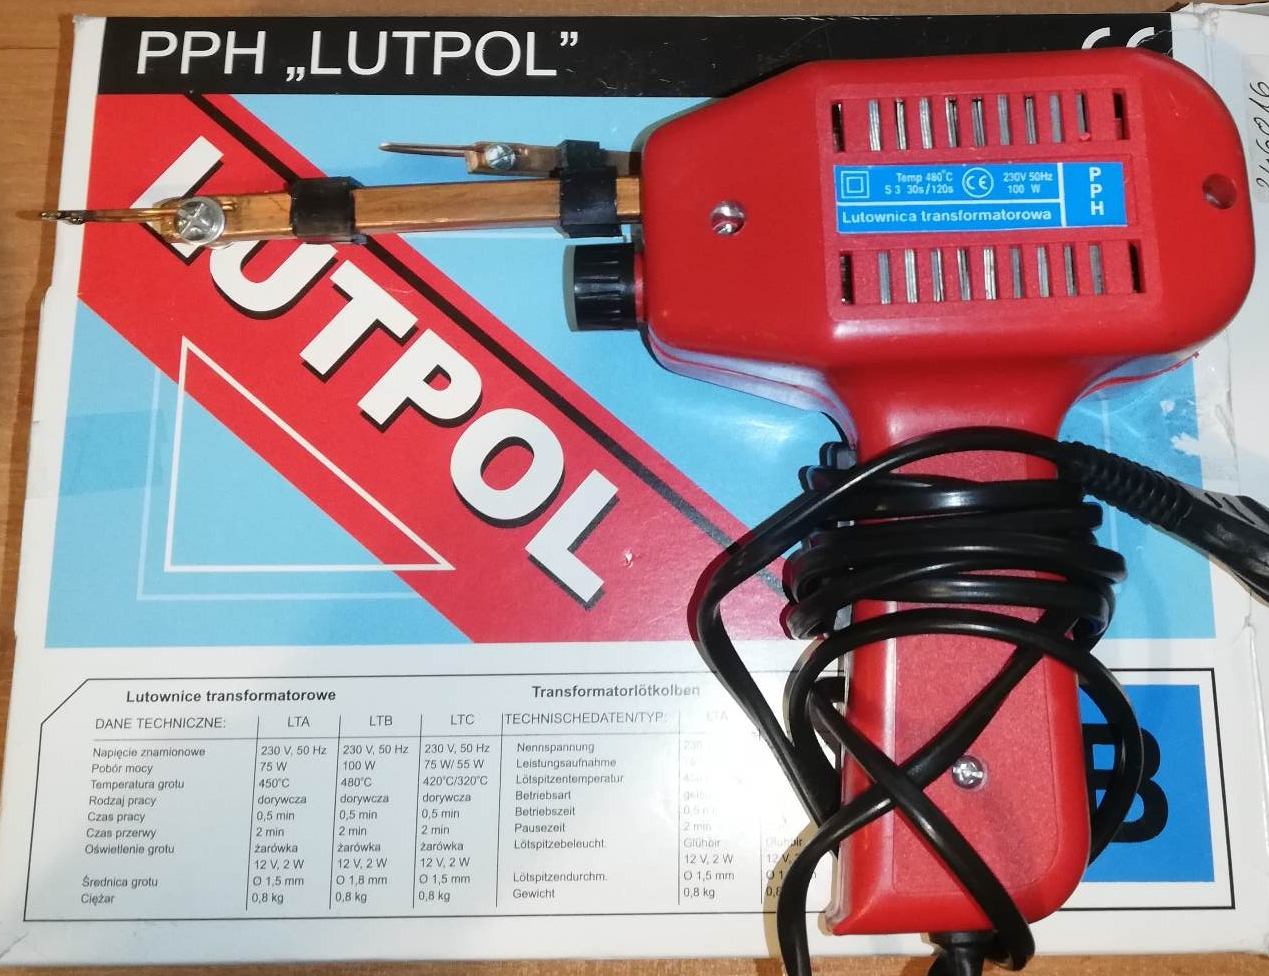
\includegraphics[scale=0.28]{images/lutownica.jpg}
    \captionof{figure}{Lutownica transformatorowa typu B}
    \label{fig:lutownica}
\end{center}

Lutownica jest najważniejszym narzędziem użytym w projekcie.

\subsubsection*{Taśma izolacyjna}
Czarna taśma izolacyjna służąca do izolacji elementów elektrycznych.

\subsubsection*{Klej na gorąco}
Pistolet do kleju posłużył do przytwierdzania elementów w miejscu (Rysunek~\ref{fig:gluegun}).

\begin{center}
    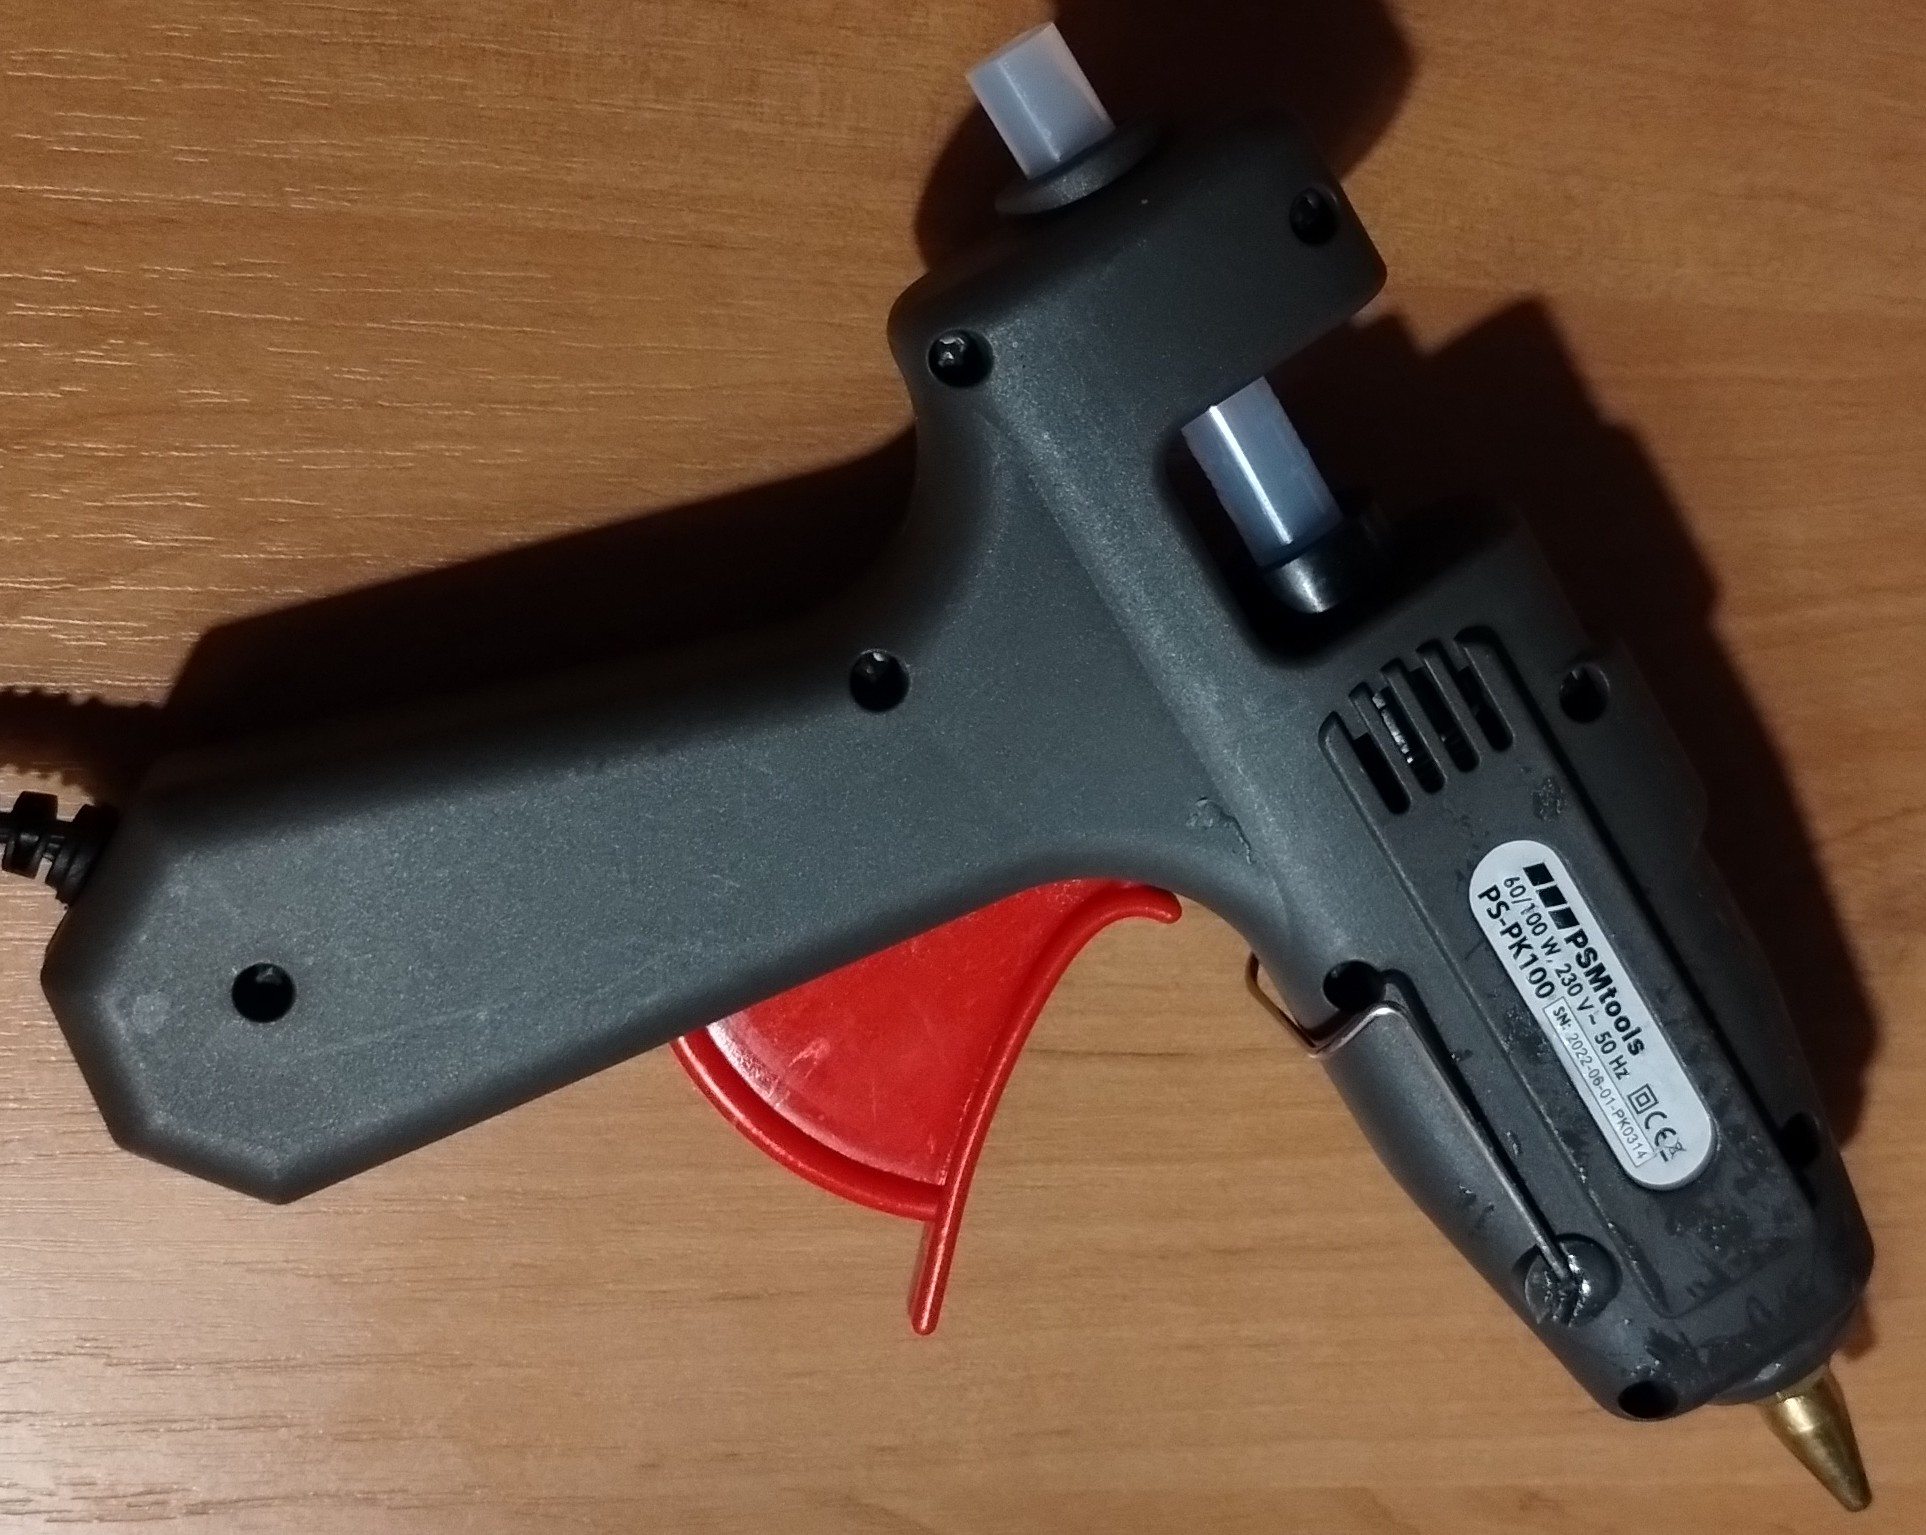
\includegraphics[scale=0.09]{images/gluegun.jpg}
    \captionof{figure}{Pistolet do kleju model PS-PK100}
    \label{fig:gluegun}
\end{center}

\subsubsection*{Multimetr}
Przyrząd pomiarowy do pomiaru wielkości elektrycznych. W projekcie użyto modelu UNI-T M830BUZ (Rysunek~\ref{fig:multimetr}) z funkcją mierzenia napięcia, natężenia, rezystancji i ciągłości.

\begin{center}
    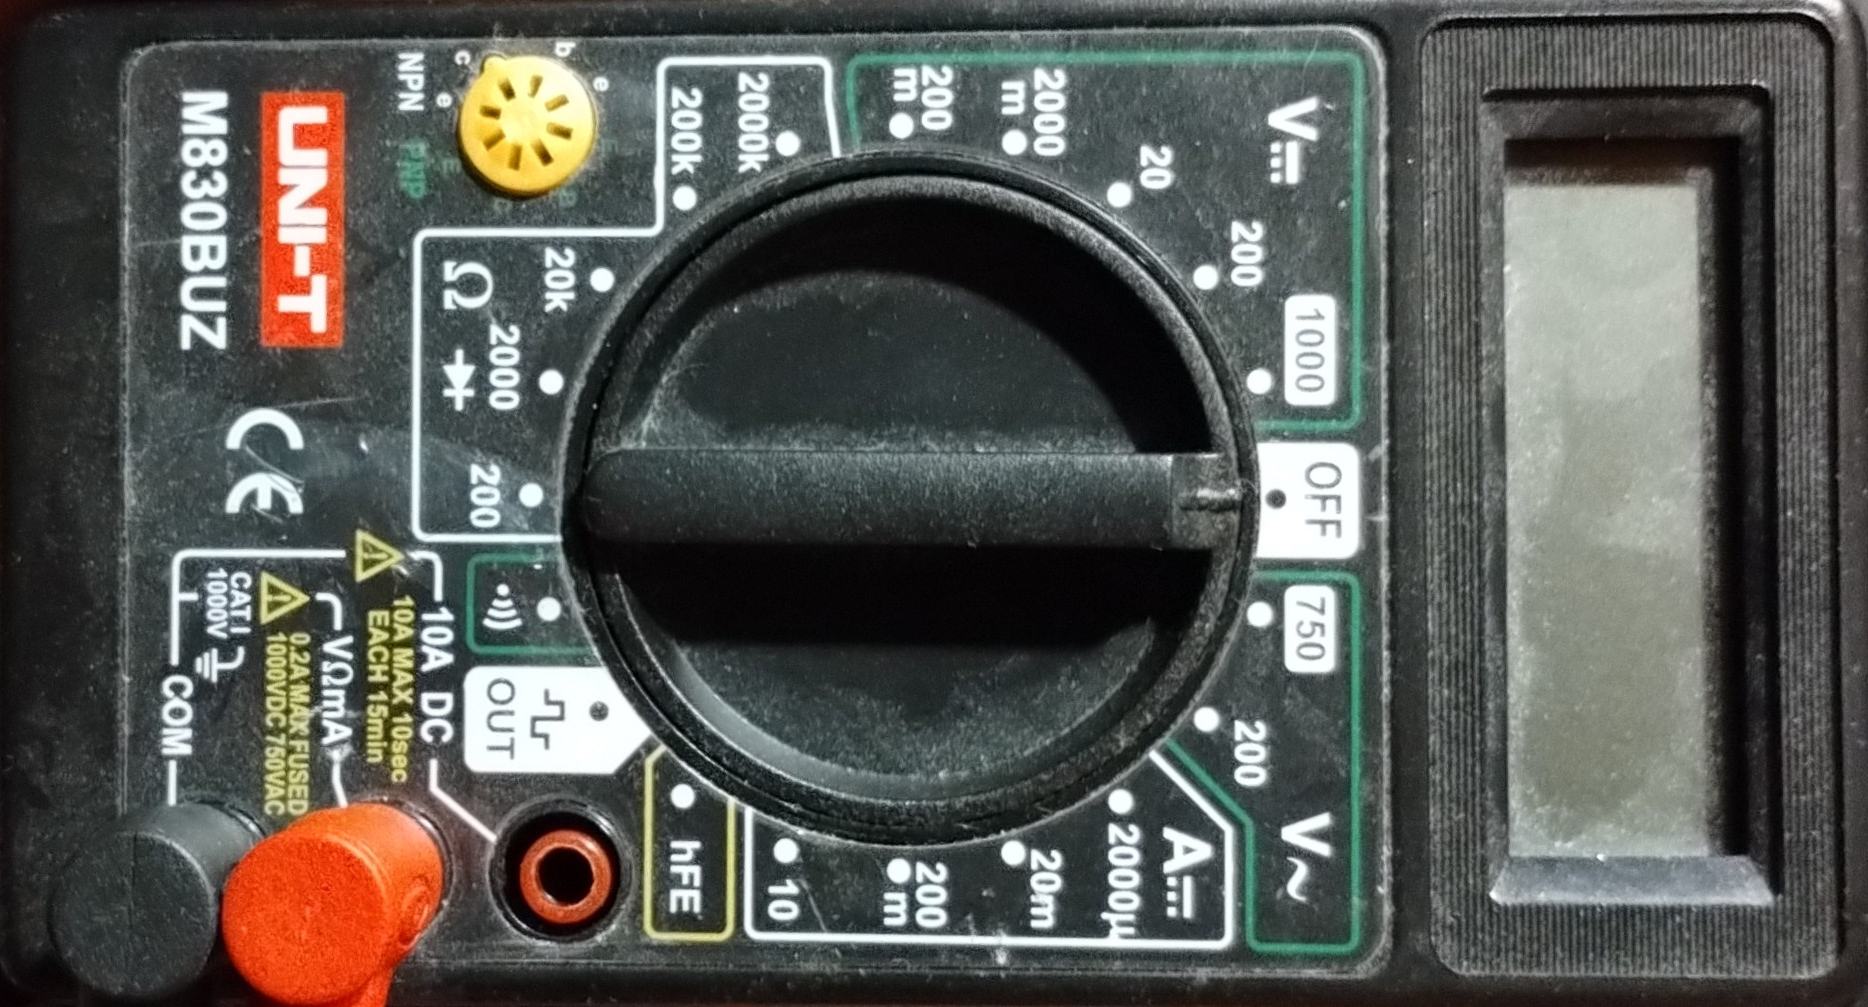
\includegraphics[scale=0.13]{images/multimetr.jpg}
    \captionof{figure}{Multimetr model UNI-T M830BUZ}
    \label{fig:multimetr}
\end{center}

\subsubsection*{Drukarka 3D}
Na drukarce 3D (Rysunek~\ref{fig:drukarka}) wydrukowano obudowę pojazdu.
\begin{center}
    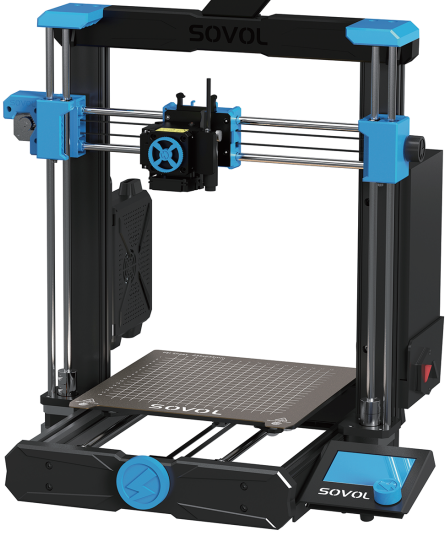
\includegraphics[scale=0.45]{images/printer.png}
    \captionof{figure}{Drukarka 3D model Sovol SV06 (Źródło:~\cite{bib:printer})}
    \label{fig:drukarka}
\end{center}

% ============ software ============ %
\subsection*{Oprogramowanie}
\subsubsection*{Visual Studio Code}
Do napisania oprogramowania mikroprocesora użyta została platforma Visual Studio Code
\begin{center}
    
\includegraphics[scale=1]{images/vscode.eps}
    \captionof{figure}{Logo platformy Visual Studio Code (Źródło:~\cite{bib:vscode})}
    \label{fig:drukarka}
\end{center}

\subsubsection*{PlatformIO}
opis
\begin{center}
    
\includegraphics[scale=0.05]{images/platformio.eps}
    \captionof{figure}{Logo platformy PlatformIO (Źródło:~\cite{bib:platformio})}
    \label{fig:drukarka}
\end{center}

\subsubsection*{MATLAB}
opis
\begin{center}
    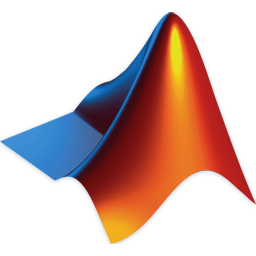
\includegraphics[scale=0.4]{images/matlab.png}
    \captionof{figure}{Logo platformy MATLAB (Źródło:~\cite{bib:matlab})}
    \label{fig:drukarka}
\end{center}

\subsubsection*{GitHub}
opis
\begin{center}
    
\includegraphics[scale=0.4]{images/GitHubLogo.eps}
    \captionof{figure}{Logo platformy GitHub (Źródło:~\cite{bib:github})}
    \label{fig:drukarka}
\end{center}